\documentclass[12pt]{article}
\usepackage[utf8]{inputenc}
\usepackage[UTF8]{ctex}
\usepackage{biblatex}
\usepackage{amssymb}
\usepackage{latexsym}
\usepackage{amsmath}
\usepackage{cases}
\usepackage{geometry}
\usepackage{graphicx}
\usepackage{float}
\usepackage{listings}
\usepackage{enumerate}
\usepackage{color}
\usepackage{hw1}



\usepackage{multirow}
\usepackage{float}
\usepackage{fancyhdr}  % header,footer的设置
\newcommand{\subsubsubsection}[1]{\paragraph{#1}\mbox{}\\}
\setcounter{secnumdepth}{4} % how many sectioning levels to assign numbers to
\setcounter{tocdepth}{4} % how many sectioning levels to show in ToC

% 封面的相关命令设置
\newcommand{\hmwkTitle}{Project 5 Solve MNA}
\newcommand{\hmwkClass}{《现代集成电路分析方法》}
\newcommand{\hmwkCompleteTime}{\today}
\newcommand{\hmwkAuthorName}{姓名:蔡志杰 }
\newcommand{\hmwMajor}{专业:电子科学与技术}
\newcommand{\hmwNumber}{学号:22112020002}
% 用fancyhdr设置header和footer
\pagestyle{fancy}
\lhead{\hmwkClass \hmwkTitle}
\rhead{蔡志杰 \quad 22112020002}
\cfoot{\thepage}


\addbibresource{bib.bib}
\setlength{\parindent}{0em}
\bibliography{bib}
\geometry{a4paper,scale=0.8}
\linespread{1.5}
\graphicspath{{Images/}}


%%%%%%%%%%%%%
%%% COVER %%%
%%%%%%%%%%%%%
\begin{document}

\begin{sloppypar}

\begin{titlepage}
\begin{center}
% \linespread{1.2}\huge {\bfseries Fudan University}\\[1cm]
% \linespread{1}
% \includegraphics[width=10cm]{fudan-name.pdf}\\[3cm]
% \linespread{1.9}\huge {\bfseries 可编程器件与硬件描述语言}\\
% \linespread{1.9}\LARGE {\bfseries 作业报告}\\[2.5cm]

% {\Large 姓名:名字}\\[0.3cm]
% \Large 学号:123456789\\[4cm] 
% \large 2021年11月1日



\includegraphics[scale = 0.9]{fudan.jpg}\\

\includegraphics[scale = 0.6]{fudan_logo.jpg}\\
\vspace{0.5in}
\linespread{1.9}\huge {\bfseries 现代集成电路分析方法}\\
\linespread{1.9}\LARGE {\bfseries \textbf{\hmwkTitle}}\\
\vspace{1.0in}
\large \hmwMajor{}\\
\large \hmwNumber{}\\
\large \hmwkAuthorName{}\\
% \large \date{\today} 

\end{center}
\end{titlepage}


\newpage
\tableofcontents
\newpage

%%%%%%%%%%%%%%%%%%%%%%%%%
%%% Problem Statement %%%
%%%%%%%%%%%%%%%%%%%%%%%%%
\section{题目}
\qquad 请设计一个程序,用后向Euler 法/梯形法求解电路系统的MNA 方程(该方程由stamp程序得到),其中线性方程的求解可以选择如下几种方法:直接法(Project III),稳态迭代法(Jacobi, G-S, SOR, Project IV),GCR迭代法(Project V)。
\begin{equation}
\label{MNA}
C \dot{X}+G X=B U
\end{equation}
\begin{equation}
Y=L^T X 
\end{equation}
系统的初值$X_0$通过求解 $GX_0 = BU(0)$ ,也就是DC分析得到。

\subsection{输入}
\qquad 输入的线性电路为SPICE格式的网表文件 \par
\qquad (1)电路方程:以提供的stamp程序的输出作为本程序的输入。 \par
\qquad (2)部分参数:模拟时间长度T,误差容限Epi。 \par
\qquad (3)电路激励:可以将源写成独立的函数,对不同的问题相应手工修改该函数,应至少支持sin以及pulse输入(关于这两种输入的具体参数请参考HSPICE手册)。 \par
\qquad (4)标准结果:以SPICE的模拟结果作为标准结果,用于和程序模拟结果比较。为方便比较结果,可以将程序的时间步长设为与SPICE一样,在时间不长不一致的情况下,则可以通过插值的方法得到在相同的时间步长下的结果。 \par

\subsection{输出结果}
\qquad 输出为四张图示和部分数值结果。 \par
\qquad 图1 为输入波形。图2 为模拟得到的输出波形。图3为模拟得到的输出波形和标准结(SPICE结果)的比较。图4为整个模拟区间上的绝对误差分布。同时程序应该输出:Euler方法的计算点数,总模拟时间,整个模拟区间上的最大绝对误差(绝对值)和均方绝对误差。 \par
\qquad * 计算误差的采样点即为标准结果中给出的时间点。如该点不是Euler方法的计算点,则模拟结果通过邻近两个计算点模拟结果的线性插值得到。 \par
\qquad ** 均方误差的定义: $MSE=\sqrt{\frac{1}{n}\sum_{i=0}^{n}E_i^2}$,其中$E_i$为每个采样点上的误差,$n$为采样点数. \par

\subsection{测试用例}
\qquad Benchmark目录下提供三个测试用例RLC\_s3.sp,bus32bit8seg.sp以及bus8bit8seg.sp,并提供Matlab下的stamp程序供构造电路矩阵。stamp用法请参考Benchmark目录下的stamp\_man文件。同时提供read\_data程序来读取hspice输出*.lis文件中的波形数据。read\_data程序的用法请参考benchmark目录下的read\_data\_man文件。Stamp程序支持sin以及pulse的输入,读取的数据在SRC变量中。\par

\subsection{提交结果}
\qquad 程序建议采用MATLAB完成,需提交以下内容: \par
\qquad (1) 源程序,应有必要的注释。 \par
\qquad (2) 使用除MATLAB外其他语言的,需要提交最终编译的可执行代码。 \par
\qquad (3) 一份完整的说明,主要内容包括:主要设计思想,程序结构,编译的环境和方法,运行的环境和方法,输入的格式或方法,以及其他需要特别说明的地方。 \par
\qquad (4) 对测试用例的测试结果和分析。 \par


%%%%%%%%%%%%%%%%%
%%% Algorithm %%%
%%%%%%%%%%%%%%%%%

\section{算法原理}

\qquad 首先通过stamp程序获得spice网表对应的电路MNA方程。对于得到电路方程,可以采用特征值分解的方法进行求解(耗时)或采用有限差分方法对其进行求解,其中有限差分法,包含前向欧拉(Forward Euler)、后向欧拉(Backward Euler)和梯形法(Trapezoidal Rule)。在有限差分法中又涉及到线性方程组的求解,求解线性方程组的方法有直接法(高斯消元法,LU分解,QR分解等)、迭代法(Jacobi,Gauss-Seidel,SOR等)和广义共轭残差法GCR。\par

\subsection{偏微分方程求解}
对于如下的偏微分方程,我们介绍前向欧拉、后向欧拉和梯形法。
\begin{equation}
  \frac{dx(t)}{dt}=Ax(t) 
\end{equation}
\begin{equation}
  x(t_0) = x_0
\end{equation}

\subsubsection{前向欧拉法Forward Euler}
前向欧拉法的公式如下,使用时间上更迟的数据点做差分来逼近梯度,只需要矩阵乘法,而不需要求解线性方程,速度更快,但是精度欠佳。
\begin{equation}
\frac{d}{d t} x\left(t_l\right)=A x\left(t_l\right) \cong \frac{x\left(t_{l+1}\right)-x\left(t_l\right)}{\Delta t}
\end{equation}
\begin{equation}
x\left(t_{l+1}\right) \cong x\left(t_l\right)+\Delta t A x\left(t_l\right)
\end{equation}
公式\ref{MNA}中前向欧拉的迭代公式为:
\begin{equation}
    CX(t_{l+1}) = (C-\Delta tG)X(t_{l}) + \Delta t BU(t_{l})
\end{equation}


\subsubsection{后向欧拉法Backward Euler}
后向欧拉法的公式如下,使用时间上更早的数据点做差分来逼近梯度,需要求解线性方程,速度慢于前向欧拉,但是精度更好。在等步长$\Delta t$的情况下,可省去重复的计算步骤来实现加速。
\begin{equation}
\frac{d}{d t} x\left(t_{l+1}\right)=A x\left(t_{l+1}\right) \cong \frac{x\left(t_{l+1}\right)-x\left(t_l\right)}{\Delta t}
\end{equation}
\begin{equation}
x\left(t_{l+1}\right) \cong x\left(t_l\right)+\Delta t A x\left(t_{l+1}\right)
\end{equation}
公式\ref{MNA}中后向欧拉的迭代公式为:
\begin{equation}
    (C+\Delta tG)X(t_{l+1}) = CX(t_{l}) + \Delta t BU(t_{l+1})
\end{equation}


\subsubsection{梯形法Trapezoidal Rule}
梯形法的公式如下,使差分来逼近相邻两点梯度的平均值,计算比后向欧拉更加复杂,但是精度更好。
\begin{equation}
  \frac{1}{2}\left(\frac{d}{d t} x\left(t_{l+1}\right)+\frac{d}{d t} x\left(t_l\right)\right)
  =\frac{1}{2}\left(A x\left(t_{l+1}\right)+A x\left(t_l\right)\right)
  =\frac{x\left(t_{l+1}\right)-x\left(t_l\right)}{\Delta t}
\end{equation}
\begin{equation}
  x\left(t_{l+1}\right)=x\left(t_l\right)+\frac{1}{2} \Delta t A\left(x\left(t_{l+1}\right)+x\left(t_l\right)\right)
\end{equation}
公式\ref{MNA}中梯形法的迭代公式为:
\begin{equation}
    (2C+\Delta tG)X(t_{l+1}) = (2C-\Delta tG)X(t_{l}) + \Delta t B(U(t_{l+1}) + U_{l})
\end{equation}

\subsubsection{小结}
\qquad 以上三种方法都是one-step方法,只依赖于前一时间点的数据。前向欧拉是最简单的方法,后向欧拉更加复杂,而梯形法可能是最精确的。

\qquad 从稳定性上看,前向欧拉的时间步长需要足够小来保证解的稳定性(极点不位于右半平面,解是等幅震荡或衰减的)。后向欧拉则能在原始解稳定的情况下保证解的稳定性,当原始解发散的时候的时候只要时间步长足够大也能保证解的衰减性。梯形法同样在解稳定时能得到稳定的解,当解不稳定(幅度不断增大时),得到的解也不稳定。

\subsection{线性方程求解}
对于如下的线性方程组,为了求解$x$的值,通常有直接法(高斯消元法,LU分解,QR分解等)、迭代法(Jacobi,Gauss-Seidel,SOR等)和广义共轭残差法GCR。

\begin{equation}
    Mx=b
\end{equation}

接下来主要迭代法和广义共轭残差法GCR.

\subsubsection{Jacobi迭代法}
\qquad 将矩阵拆分成上三角、对角线和下三角矩阵,通过移项得到迭代公式:
\begin{equation}
    M=D-L-U
\end{equation}
\begin{equation}
    (D-L-U)x=b
\end{equation}
\begin{equation}
    Dx_k=(U+L)x_{k-1}+b
\end{equation}

\qquad 迭代速度较慢,没有合理利用前面迭代得到的信息。
\subsubsection{Gauss-Seidel迭代法}
\qquad 和Jacobi方法相比,利用了更多先前迭代中的结果,能获得更快的收敛速度:
\begin{equation}
    (D-L)x_k=Ux_{k-1}+b
\end{equation}
\subsubsection{Successive Over Relaxation逐次超松弛法}
\qquad 基于Guass-Seidel迭代法,进行修改来提高迭代收敛速度,
\begin{equation}
  x_k = w\overline{x_k} + (1+w)x_{k-1}
\end{equation}
\begin{equation}
  \overline{x_k} = D^{-1}Lx_k + D^{-1}Ux_{k-1} + D^{-1}b
\end{equation}
\begin{equation}
  x_k = (D-wL)^{-1}((1-w)D+wU)x_{k-1} + w(D-wL)^{-1}b
\end{equation}

\subsubsection{广义共轭残差法GCR}
\qquad 第$k$轮残差的定义为,
\begin{equation}
  r^k \equiv b - Mx^k
\end{equation}

\qquad 第k轮迭代的解$x_k$定义为,
\begin{equation}
  x^{k+1} = \sum_{i=0}^{k} \alpha_i w_i
\end{equation}
\qquad 目标是最小化残差的2范数,当构成$x$的基向量关于$M$矩阵正交,即$(Mw_i)^T(Mw_j)=0(i\neqj)$时残差的2范数很容易优化,
\begin{equation}
  \mathop{\min}_{x} \Vert r^{k+1} \Vert_2^2 = \Vert b - \sum_{i=0}^{k} \alpha_i M w_i \Vert
\end{equation}
\qquad 将其转换成一个二次型目标函数,取最优值的地方梯度为0,梯度对应的就是残差,能够间接求解线性方程组。(只适用于矩阵$M$为对称正定阵)
\begin{equation}
  f(x) = \frac{1}{2}x^TMx-x^Tb
\end{equation}
\begin{equation}
  \triangledown_xf(x) = Mx-b
\end{equation}
\qquad 对目标函数f采用最速下降法,将梯度作为新的探索方向,经过分析可得如下的迭代公式:
\begin{equation}  
  \alpha_k= \frac{\left(r^k\right)^T\left(M p_k\right)}{\left(M p_k\right)^T\left(M p_k\right)} 
\end{equation}
\begin{equation}
  x^{k+1} =x^k+\alpha_k p_k
\end{equation}
\begin{equation}
  r^{k+1} =b-M x^{k+1} =b-M x^k-\alpha_k M p_k =r^k-\alpha_k M p_k
\end{equation}
\begin{equation}
  p_{k+1} =r^{k+1}-\sum_{j=0}^k \frac{\left(M r^{k+1}\right)^T\left(M p_j\right)}{\left(M p_j\right)^T\left(M p_j\right)} p_j
\end{equation}
\qquad 如果矩阵$M$是稀疏的,具有$k$个特征值,你们只需要$k$轮迭代即可收敛,收敛速度更快。当矩阵$M$为对称矩阵时,$r^{k-1} \bot Mp_j,j<k$,$p_{k+1}$的正交化只需要一步操作。
\begin{equation}
  p_{k+1}=r^{k+1}-\sum_{j=0}^k \frac{\left(M r^{k+1}\right)^T\left(M p_j\right)}{\left(M p_j\right)^T\left(M p_j\right)} p_j \Rightarrow p_{k+1}=r^{k+1}-\frac{\left(M r^{k+1}\right)^T\left(M p_k\right)}{\left(M p_k\right)^T\left(M p_k\right)} p_k
\end{equation}

\section{算法实现}

\subsection{算法流程}
\qquad 算法流程
\begin{itemize}
  \item 使用提供的stamp动态库对hsipce网表进行解析得到相应的矩阵数据,使用hspice进行仿真,得到相应的波形lis文件,调用read\_data函数来得到相应lis文件中hspice仿真的波形结果。(main.m)
  \item 根据stamp解析到的输入信号信息生成相应的激励信号数据。(GenerateSrc.m)
  \item 根据函数的输入选择是使用Backward Euler还是Trapezoidal Rule的方法来求解偏微分方程。(BackwardEuler.m, TrapezoidalRule.m)
  \item 在Backward Euler还是Trapezoidal Rule中根据函数的输入决定采用GCR还是SOR进行线性方程的求解。(GCR.m, SOR.m)
  \item 将得到的仿真结果通过线性插值得到与hspice相同采样时间的数据点,并计算相应的误差(最大绝对误差和均方绝对误差)。(main.m)
  \item 生成结果对比图。(report.m)
\end{itemize}


\subsection{输入激励信号}
\qquad 脉冲源

\qquad 语法:

\qquad Vxxx n+ n- PU<LSE> <(>v1 v2 <td <tr <tf <pw <per> > > > > <)>

\qquad Ixxx n+ n- PU<LSE> <(>v1 v2 <td <tr <tf <pw <per> > > > > <)>

\qquad 其中v1为脉冲源的低压,v2为高压,td为延迟,tr为上升时间,tf为下降时间,pw为脉冲宽度,per为信号周期。下图展示了一个脉冲信号源的例子:

\begin{figure}[H]
  \centering
  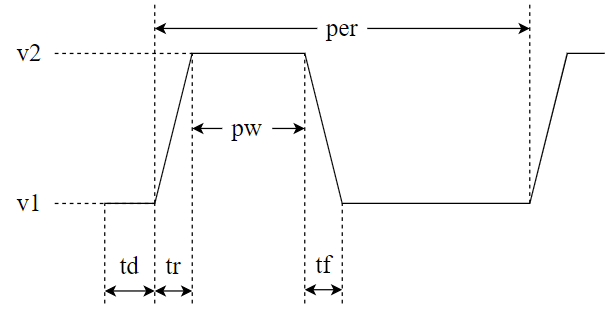
\includegraphics[width=0.5\columnwidth]{figure/pulse.png}
  \caption{脉冲信号源示例}
\end{figure}

\qquad 正弦源

\qquad 语法:

\qquad Vxxx n+ n- SIN <(> vo va <freq <td <$\theta$ <$\phi$> > > > <)>

\qquad Ixxx n+ n- SIN <(> vo va <freq <td <$\theta$ <$\phi$> > > > <)>

\qquad 其中vo为直流幅度,va为交流幅度,freq为频率,td为延时,$\theta$为衰减因子,$\phi$为相位延时。信号的公式可以如下:

\begin{equation}
  y(t) = e^{-\theta}\cdot va \cdot sin(2\pi \cdot freq \cdot(t-td) - \phi) + vo
\end{equation}


\subsection{线性方程组求解}
\qquad 不论是使用GCR还是SOR来求解线性方程组都需要确定一个误差容限,本实验中将误差容限$errorThres$的设置放到顶层函数接口,同时误差的标准为两次迭代间解$x$值的变化的2范数,即:

\begin{equation}
  ||x_{t+1} - x_{t}|| < errotThres
\end{equation}

\qquad 此外迭代的轮数也要进行限制,GCR迭代的最大轮数即为矩阵的行/列数,SOR的最大迭代轮数设置成1000轮。

\subsection{输出}
\qquad 为了将仿真结果与hspice的结果进行对比,首先需要通过插值法得到自己仿真结果在hspice采样时间上的值,然后求解最大绝对误差和均方绝对误差。同时为了方便访问结果,使用save命令将仿真的数据存储到.mat文件中。对于有多个输出节点的电路,为了方便观察选取其中一个的波形进行绘制。

\section{编译与运行}
\qquad 程序基于Matlab 2015b(32位)平台,将整个解析网表文件、MNA方程求解和结果输出的过程都打包在main函数中,由于所有benchmark都在Benchmark目录中,所以需要在matlab中将当前目录切换到Benchmark下运行。main函数的接口为$main(caseName, methodName,algorithmName, startTime, endTime, stepNum, errorThres)$. 其中caseName(RCL\_s3, RCL\_p3,bus8bit8seg,bus32seg16),methodName(BE,TR), \\ algorithmName(SOR,GCR)分别对于测试用例名、常微分方程求解方法(后向欧拉和梯形法),以及线性方程求解方法。startTime和endTime为记录仿真结果的时间区间,stepNum为这一区间的采样数,errorThres为误差阈值。下面给出一个运行示例:

\begin{equation}
  main('RLC_s3','BE','GCR',0 ,2e-2,1000,1e-9)
\end{equation}

\section{结果与分析}
\subsection{实验结果}
\subsubsection{RLC\_s3(正弦激励信号)}
\qquad 仿真设置:起始时间0s,终止时间0.02s,采样点数1000,误差容限$1e^{-9}$,输入的正弦信号激励为$3sin(400\pi t)$。下面展示了几种算法得到的仿真结果:

后向欧拉(BE)+GCR:

\begin{figure}[H]
  \centering
  \includegraphics[width=0.7\columnwidth]{figure/RLC\_s3\_BE\_GCR.png}
  \caption{RLC\_s3\_BE\_GCR实验结果}
\end{figure}

梯形法(TR)+GCR:

\begin{figure}[H]
  \centering
  \includegraphics[width=0.7\columnwidth]{figure/RLC\_s3\_TR\_GCR.png}
  \caption{RLC\_s3\_TR\_GCR实验结果}
\end{figure}

后向欧拉(BE)+SOR:

\begin{figure}[H]
  \centering
  \includegraphics[width=0.7\columnwidth]{figure/RLC\_s3\_BE\_SOR.png}
  \caption{RLC\_s3\_BE\_SOR实验结果}
\end{figure}

梯形法(TR)+SOR:

\begin{figure}[H]
  \centering
  \includegraphics[width=0.7\columnwidth]{figure/RLC\_s3\_TR\_SOR.png}
  \caption{RLC\_s3\_TR\_SOR实验结果}
\end{figure}

\subsubsection{RLC\_p3(脉冲激励信号)}
\qquad 仿真设置:起始时间0s,终止时间0.02s,采样点数1000,误差容限$1e^{-9}$,输入的方波信号为周期为20ms,高低电平分别为3V和0V,上升下降时间为1ms,高电平时间为3ms,信号延迟为1ms。下面展示了几种算法得到的仿真结果:

后向欧拉(BE)+GCR:

\begin{figure}[H]
  \centering
  \includegraphics[width=0.7\columnwidth]{figure/RLC\_p3\_BE\_GCR.png}
  \caption{RLC\_p3\_BE\_GCR实验结果}
\end{figure}

梯形法(TR)+GCR:

\begin{figure}[H]
  \centering
  \includegraphics[width=0.7\columnwidth]{figure/RLC\_p3\_TR\_GCR.png}
  \caption{RLC\_p3\_TR\_GCR实验结果}
\end{figure}

后向欧拉(BE)+SOR:

\begin{figure}[H]
  \centering
  \includegraphics[width=0.7\columnwidth]{figure/RLC\_p3\_BE\_SOR.png}
  \caption{RLC\_p3\_BE\_SOR实验结果}
\end{figure}

梯形法(TR)+SOR:

\begin{figure}[H]
  \centering
  \includegraphics[width=0.7\columnwidth]{figure/RLC\_p3\_TR\_SOR.png}
  \caption{RLC\_p3\_TR\_SOR实验结果}
\end{figure}

\subsubsection{bus8bit8seg(脉冲激励信号)}
\qquad 仿真设置:起始时间0s,终止时间$1e^{-9}$s,采样点数1000,误差容限$1e^{-9}$,输入的方波信号为周期为0.5ns,高低电平分别为1V和0V,上升下降时间为0.05ns,高电平时间为0.3ns,信号延迟为0.05ns。下面展示了几种算法得到的仿真结果:

后向欧拉(BE)+GCR:

\begin{figure}[H]
  \centering
  \includegraphics[width=0.7\columnwidth]{figure/bus8bit8seg\_BE\_GCR.png}
  \caption{bus8bit8seg\_BE\_GCR实验结果}
\end{figure}

梯形法(TR)+GCR:

\begin{figure}[H]
  \centering
  \includegraphics[width=0.7\columnwidth]{figure/bus8bit8seg\_TR\_GCR.png}
  \caption{bus8bit8seg\_TR\_GCR实验结果}
\end{figure}

\subsubsection{bus32seg16(脉冲激励信号)}
\qquad 仿真设置:起始时间0s,终止时间$1e^{-9}$s,采样点数1000,误差容限$1e^{-9}$,输入的方波信号为周期为0.5ns,高低电平分别为1V和0V,上升下降时间为0.05ns,高电平时间为0.3ns,信号延迟为0.05ns。下面展示了几种算法得到的仿真结果:

后向欧拉(BE)+GCR:

\begin{figure}[H]
  \centering
  \includegraphics[width=0.7\columnwidth]{figure/bus32seg16\_BE\_GCR.png}
  \caption{bus32seg16\_BE\_GCR实验结果}
\end{figure}

梯形法(TR)+GCR:

\begin{figure}[H]
  \centering
  \includegraphics[width=0.7\columnwidth]{figure/bus32seg16\_TR\_GCR.png}
  \caption{bus32seg16\_TR\_GCR实验结果}
\end{figure}

\subsection{结果分析}

\qquad 从上述结果中可以看出在给定的电路已经仿真条件下使用后向欧拉法和梯形法得到的误差相差不大,运行时间上也没有显著的差异,分析原因可能是电路本身都是稳定的,同时由于实现过程中Matlab底层对矩阵不同运算处理的优化上不同。此外SOR和GCR两种求解线性方程组的方法在RLC的例子上表现相当,但是SOR的收敛轮数会大于GCR的收敛轮数,此外还尝试使用了matlab自带的线性方程求解方法(于golden.m文件中),得到的结果与GCR,SOR相近,同时运行时间明显更快,可见matlab自带的线性方程求解器的高效。

\section{文件说明}
\qquad src目录中的文件结构
\begin{itemize}
  \item main.m:包含整个MNA方程的求解框架和流程。
  \item BackwardEuler.m:实现后向欧拉求解法。
  \item TrapezoidalRule.m:实现梯形法。
  \item GCR.m:实现GCR算法。
  \item SOR.m:实现SOR算法。
  \item Golden.m:使用matlab自带线性方程求解器进行求解。
  \item GenerateSrc.m:生成激励信号。
  \item report.m:分析数据并绘制对比图。
\end{itemize}

\end{sloppypar}
\end{document}